\documentclass[
  journal=medium,
  manuscript=article-type,
  year=2023,
  volume=37,
]{cup-journal}

\usepackage{amsmath}
\usepackage[nopatch]{microtype}
\usepackage{booktabs}
\usepackage{graphicx}
\usepackage[UTF8]{ctex}


\title{基于电商平台的女装在线评论数据挖掘及情感分析}

\author{杨雨潇}
\affiliation{西安交通大学,西安,中国}
\email[杨雨潇]{2201111610@xjtu.edu.cn}

\addbibresource{example.bib}

\keywords{电商平台,在线评论,数据探索性分析,Logistic,LightGBM} %% First letter not capped

\begin{document}

\begin{abstract}

    本文对某电商平台女士服装在线评论数据进行建模,包括文本进行预处理、探索性分析-单变量探索和多变量联合探索、英文分词并用停用词过滤、基于VADER的情绪分析模型、基于Logistic和Lightgbm算法的预测模型,从多个方面对电商评论数据进行了分析,为电商平台提供客户画像及情绪分析,可供辅助营销决策。

\end{abstract}



\section{引言}

随着电子商务行业的快速发展,网络购物变得越来越流行,销售模式由线下向线上逐渐转变,传统的营销模式面临改变。电商在线评论数据对消费者和商家都具有非常重要的价值,购买者通过各种电商平台平台购买商品,并对商品进行评论以表达对购物体验及商品性能的满意程度,同时,人们往往在购买商品之前,除了查看商品信息, 也会浏览该商品的评论,从其他已购买的顾客评论中获取有价值的信息。因此,在人们无法看到具体实物时,评论成为了一个重要的参考渠道,影响着人们的购买决策。评论对商家也具有应用价值,顾客对商品的真实反馈可以帮助商家制定今后的商品改进或营销策略,而对在线评论进行文本情感分析可以有效提炼消费者体验信息和产品相应属性的评价观点,从而最直观地体现用户的需求和关注点,值得关注的是,在线评论数据不仅仅是评论文本内容,还包括评论的点赞数量、用户是否愿意推荐、用户的个人信息等等,获取这些信息有助于更深入理解消费者行为。由于女士更愿意在社交平台、电商平台上评论分享,并且其评论内容注重个体感受,因此女士服装是良好的研究领域。本文基于某匿名电商平台的女士服装在线评论数据,试图通过数据探索性分析、情绪分析、预测分析得到一些具有业务价值的信息,为电商平台提供相应的对策与建议。

\section{研究背景}

评论文本数据与普通文本数据不同,评论不仅包含主题,还包含主观性的情感色彩,书写形式也不规范,具有口语化的特点,如何在挖掘主题的同时, 进行情感分析成为一个难题。 情感是人们对商品的态度,是人们通过文本表达出的情绪,一般分为两种积极或消极,积极说明对这一属性较为满意,消极则是对商品的某一方面不满,没有达到预期。学者们认为用户评论具有高度的分析价值,虽然其研究角度各有不同,但都取得了一定的研究成果。在已有的研究中,一些学者主要从特征提取、情感分析等方面进行了研究。目前主流的文本挖掘模型有LDA(主题生成模型)、最大熵模型,对于关键词提取方法,有tf-idf、bm25、textrank、pagerank、互信息和左右熵等,对于词法分析,有HMM、CRF、词性标注、命名实体识别等,对于句法,有句法结构分析和依存句法分析,对于文本向量化,主流方法有tf-idf、word2vec、doc2vec、cw2vec等等。

\section{样本数据}

\subsection{数据来源}

本数据源自2016年某海外电商平台,为真实数据,由 nicapotato 爬虫爬取并经过脱敏化处理,整理后发布在Kaggle平台上。

\subsection{数据描述}

\subsubsection{元数据描述}

该数据集包括23486行和10个特征变量。每一行为一个用户的评论,每一列为一个特征变量,详细说明见 表~\ref{attribute}

\begin{table}[hbt!]
    \begin{threeparttable}
    \caption{元数据}
    \label{attribute}
    \begin{tabular}{lll}
    \toprule
    \headrow 特征名称 & 特征描述 & 特征类型\\
    \midrule
    Clothing ID & 服装标签 & 整数类别变量 \\ 
    \midrule
    Age & 评论者年龄 & 正整数变量\\ 
    \midrule
    Title & 评论标题 & 字符串变量\\ 
    \midrule
    Review Text & 评论内容 & 字符串变量\\ 
    \midrule
    Rating & 产品评价打分 & 正序整数变量,从1(最差)到5(最佳)\\ 
    \midrule
    Recommended IND & 评论者是否推荐某服装 & 正整数0-1变量,其中1为推荐,0为不推荐\\ 
    \midrule
    Positive Feedback Count & 该评论得到其他用户积极认可的数量(评论点赞) & 正整数变量\\ 
    \midrule
    Division Name & 产品类别 & 字符串变量\\ 
    \midrule
    Department Name & 服饰类别 & 字符串变量\\ 
    \midrule
    Class Name & 服饰类型 & 字符串变量\\ 
    \bottomrule 
    \end{tabular}
    \end{threeparttable}
\end{table}
    
    
\subsubsection{数据统计性描述}   

$\bullet$数值变量:

通过对数值变量的简单统计性描述(表~\ref{table_describe_number}),对于Age-年龄,我们发现评论者年龄平均为43岁左右;对于Rating-产品评价打分,其平均在4.2分,满分为5分,分数较高,通过观察四分位数,我们可以简单得出其分布为左偏分布;对于Recommended IND-是否推荐,其平均分为0.822,通过观察四分位数,我们也可以简单得出其分布为左偏分布,可能与Rating-产品评价打分具有较强的正相关性;对于Positive Feedback Count-评论点赞,其标准差较大,说明数据分布波动较大,同时其分布为右偏分布。

\begin{table}[hbt!]
    \begin{threeparttable}
    \caption{数值型变量统计性描述}
    \label{table_describe_number}
    \begin{tabular}{llllllll}
    \toprule
    \headrow 特征名称 & 平均值 & 标准差 & 最小值 & 1/4 四分位数 & 1/2 四分位数 & 3/4 四分位数 & 最大值\\
    \midrule
    Clothing ID & 918.118709 & 203.298980 & 0.0 & 861.0 & 936.0 & 1078.0 & 1205.0 \\ 
    \midrule
    Age & 43.198544 & 12.279544 & 18.0 & 34.0 & 41.0 & 52.0 & 99.0 \\
    \midrule
    Rating & 4.196032 & 1.110031 & 1.0 & 4.0 & 5.0 & 5.0 & 5.0 \\
    \midrule
    Recommended IND & 0.822362 & 0.382216 & 0.0 & 1.0 & 1.0 & 1.0 & 1.0 \\
    \midrule
    Positive Feedback Count & 2.535936 & 5.702202 & 0.0 & 0.0 & 1.0 & 3.0 & 122.0 \\
    \bottomrule 
    \end{tabular}
    \end{threeparttable}
\end{table}



$\bullet$字符型变量:

通过对字符型变量的简单统计性描述(表~\ref{table_describe_str}),对于Title-评论标题,出现频次最高的数据为正向情绪,出现了136次;对于Review Text-评论内容,其内容多为不重复,这也在预期之中,因为评论内容具有较长的长度,出现重复的可能性也小;对于剩下三个特征,我们分别可以得知其出现频次最高的数据的出现频次。分别为13850、10468、6319次。

\begin{table}[hbt!]
    \begin{threeparttable}
    \caption{字符型变量统计性描述}
    \label{table_describe_str}
    \begin{tabular}{llll}
    \toprule
    \headrow 特征名称 & 不重复数据数量 & 频次最高数据 & 频次\\
    \midrule
    Title & 13993 & Love it! & 136 \\ 
    \midrule
    Review Text & 22634 & Perfect fit and i've gotten so many compliment... & 3 \\ 
    \midrule
    Division Name & 3 & General & 13850 \\ 
    \midrule
    Department Name & 6 & Tops & 10468 \\
    \midrule
    Class Name & 20 & Dresses & 6319 \\
    \bottomrule 
    \end{tabular}
    \end{threeparttable}
\end{table}


\subsection{数据预处理}  

$\bullet$缺失值处理:

由缺失值矩阵图和柱状图(图~\ref{fig_missing_distribute} 和 图~\ref{fig_missing_bar})我们发现Title-标题数据缺失较为严重,Review Text-评论内容也有一定程度的缺失。在23486条数据中缺损值分别为:Title-标题 3810条,Review Text-评论内容 845条,Division Name-产品类别、Class Name-服饰类别 、Department Name-服饰类型各14条。

对于缺失值的处理,由于Review Text-评论内容是分析的重点,无法通过其他方法补充,同时Division Name-产品类别、Class Name-服饰类别 、Department Name-服饰类型仅凭服装的ID无法获取,因此将该四个特征的所有缺失值所在的行删去。而Title-标题由于缺失数据量较大,占整体数据的百分之16,不能将其简单删除,如若将其与Review Text-评论内容结合,又无法探索Title本身的信息,因此在此处先对其进行保留不处理,删除后,共有2966个缺失值,共有22628行数据。

\begin{figure}[hbt!]
    \centering
    \includegraphics[width=1.0\linewidth]{缺失值分布.png}
    \caption{数据缺失值分布}
    \label{fig_missing_distribute}
\end{figure}

\begin{figure}[hbt!]
    \centering
    \includegraphics[width=1.0\linewidth]{缺失值柱状图.png}
    \caption{缺失值柱状图}
    \label{fig_missing_bar}
\end{figure}



\subsection{特征提取} 

观察特征变量,由于Title-标题和Review Text-评论内容为字符型变量,无法与其他数值型变量同时分析,因此可以添加描述字符型变量的特征变量,如对Title-标题和Review Text-评论内容的用词数量或者英文字母数量进行分析,因此在此基础上添加了两个新的特征,分别为Review Text-评论内容的用词数量(Word Count)和英文字母数量(Character Count);同时,为了便于之后进行自然语言的监督模型分类训练,我们需要将Rating-产品评价打分二值化,即归纳为好和不好;值得一提的是,虽然Recommended IND-是否推荐是二值0-1变量,但是该变量更能反映的是产品的社会性,即某个服装可能不适合评论者自身,但是它总体上是值得推荐给别人的,这就有悖于我们对产品评价打分的归纳;我们将大于等于3分的打分编码为1,小于3分的打分编码为0。

关于新提取特征的统计性描述分析:

\begin{table}[hbt!]
    \begin{threeparttable}
    \caption{新提取特征统计行描述}
    \label{table_describe_new}
    \begin{tabular}{llllllll}
    \toprule
    \headrow 特征名称 & 平均值 & 标准差 & 最小值 & 1/4 四分位数 & 1/2 四分位数 & 3/4 四分位数 & 最大值\\
    \midrule
    Word Count & 60.211950 & 28.533053 & 2.0 & 36.0 & 59.0 & 88.0 & 115.0  \\ 
    \midrule
    Character Count & 308.761534 & 143.934126 & 9.0 & 186.0 & 302.0 & 459.0 & 508.0 \\
    \midrule
    Label & 0.895263 & 0.306222 & 0.0 & 1.0 & 1.0 & 1.0 & 1.0  \\
    \bottomrule 
    \end{tabular}
    \end{threeparttable}
\end{table}

\section{数据探索} 

\subsection{单变量数据探索} 

$\bullet$\textbf{Age-年龄和Positive Feedback Count-评论点赞分布:}

对年龄和评论点赞数量进行直方图可视化(图~\ref{age_Feedback}),可以发现电商评论中主要评论者为40岁左右的中年女性,呈现轻微的右偏分布,这与我们通常认为的电商消费评论者主要为年轻女性有些出入;同时,Positive Feedback Count-评论点赞数量好似呈现指数形式,大多数评论者都得到了极为少量的点赞,进一步研究,我对其先进行了平滑处理,之后取对数,探究其变化是否为指数,结果显示经过取对数后还有基本呈线性关系,这基本符合我们平常认为的分布,即少量的人占据着大量的资源,即二八定律,大多数都是低于平均值的。

\begin{figure}[hbt!]
    \centering
    \includegraphics[width=1.0\linewidth]{age_positivefeedback.pdf}
    \caption{年龄和评论点赞分布}
    \label{age_Feedback}
\end{figure}

对Positive Feedback Count-评论点赞数量进行进一步的分析,自变量为当前评论者的累计百分比,排序由Positive Feedback Count-评论点赞数量降序排序,因变量为当前评论点赞数量的累计百分比,得到的结果如图~\ref{28},我们可以发现,前百分之20的评论者拥有百分之78的点赞量,这几乎完美印证了二八定律,同时,我们计算Positive Feedback Count-评论点赞数量变量的基尼系数,其值为0.76,基尼系数越靠近1,说明其不平均的程度越大;极少部分评论者的评价获得了大量的评论点赞,该部分评论者可能是最早期评论者,或者是其评论十分出彩,得到了大多数人的赞同而大多数人(约百分之47)没有任何评论点赞。

\begin{figure}[hbt!]
    \centering
    \includegraphics[width=0.6\linewidth]{28.pdf}
    \caption{评论点赞累计百分比图}
    \label{28}
\end{figure}

$\bullet$\textbf{Rating-打分、Recommended IND-是否推荐和 Label-标签分布:}

对评价打分、是否推荐和标签进行频数分布图可视化(图~\ref{Rating_Recommended_Label}),通过Rating-打分,可以发现该服装店商的打分从5到1的数量逐渐减少,说明其店铺业绩表现很好,同时,通过是否推荐和Label-标签和可以发现绝大部分的评分较高,客户的满意度较高,愿意将该商品分享给自己的亲友,分享到社会,说明该店铺的营销方案是相当成功的。


\begin{figure}[hbt!]
    \centering
    \includegraphics[width=1.1\linewidth]{3feature.pdf}
    \caption{打分、是否推荐和标签分布}
    \label{Rating_Recommended_Label}
\end{figure}

$\bullet$\textbf{Division Name-产品类别和Department Name-服饰类别分布:}

对产品类别和服饰类别进行频数分布图可视化(图~\ref{Name}),通过Division Name-产品类别柱状图,可以发现购买普通款式的消费者最多,小款数量其次,亲密款消费者最少,这位我们构建用户画像提供了基础;通过Department Name-服饰类别柱状图,可以发现上衣和连衣裙是评论数量最多的服饰类别,可以基于此研究这两种服饰类别的评论动机。对于Class Name-服饰类型,由于其类型较多,因此放在多变量分布分析中进行。

\begin{figure}[hbt!]
    \centering
    \includegraphics[width=1.1\linewidth]{2feature_Name.pdf}
    \caption{产品类别和服饰类别分布}
    \label{Name}
\end{figure}


\subsection{多变量数据联合探索} 

$\bullet$\textbf{特征变量的相关性分析}

计算数值型变量间的pearson相关性并以热力图可视化(图~\ref{corr}),可以发现Label-标签与Rating-打分具有强相关性,通过Label-标签特征的生成方式我们也可以推出;同时,Rating-打分和Recommended IND-是否推荐也具有强相关性,可以推出打分高的评论者更愿意将产品推荐给他人,而打分低的评论者更不愿意将产品推荐给他人;同时Word Count-用词数量和Character Count-英文字母数量与Positive Feedback Count-评论点赞数量有弱相关性,可以推出评论内容的用词数量和评论点赞数量有弱正相关关系。值得关注的是,各特征之间没有强负相关关系。

$\bullet$\textbf{基于不同Class Name-服饰类型的平均年龄与是否推荐可能性的相关性分析:}

经过研究各特征变量的相关性后,我选择了某个离散分类变量,研究在不同Class Name-服饰类型的平均年龄与是否推荐可能性的相关性分析;计算不同服饰类型下平均年龄与是否推荐可能性的pearson相关性并以热力图可视化(图~\ref{corr2}),可以发现推荐可能性-Recommended Likelihood与平均年龄-Age Mean 有强负相关性关系,为了进一步研究关系,可视化了推荐可能性与平均年龄的散点图(图~\ref{corr3}),可以发现随着年龄的增加,不同服饰类型的推荐可能性会降低;但这并不是因果关系,可能是因为某些服饰类型针对的年龄段不同,同时其对于消费者的体验也不同,比如阿迪达斯kids针对的主要年龄段是童龄,其童装年龄打分也较高,而店内的一些其他物品(不针对儿童),受众年龄较大,同时由于不是主要产品,其打分可能较低。

\begin{figure}[hbt!]
    \centering
    \includegraphics[width=0.8\linewidth]{corr.pdf}
    \caption{各特征间的相关系数热力图}
    \label{corr}
\end{figure}

\begin{figure}[H]
    \centering
    \includegraphics[width=0.8\linewidth]{corr2.pdf}
    \caption{基于不同服饰类型的相关系数热力图}
    \label{corr2}
\end{figure}


\begin{figure}[hbt!]
    \centering
    \includegraphics[width=0.6\linewidth]{corr3.pdf}
    \caption{平均年龄与推荐可能性散点图}
    \label{corr3}
\end{figure}


$\bullet$\textbf{基于不同Rating-打分、Recommended IND-是否推荐、Division Name-服饰类别、Class Name-服饰类型的Age-年龄频数分布}

基于不同的特征变量对年龄进行频数可视化(图~\ref{age_others}),在不同的特征取值下,年龄分布均无明显差异,说明打分、是否推荐、服饰类别、服饰类型等特征均与评论者年龄无相关关系,特征变量的变化不会影响年龄分布。

\begin{figure}[hbt!]
    \centering
    \includegraphics[width=1.1\linewidth]{age_others.pdf}
    \caption{基于不同特征取值的年龄分布}
    \label{age_others}
\end{figure}

$\bullet$\textbf{Division Name-产品类别和Class Name-服饰类型的交叉透视表}

对产品类别和服饰类别进行频数与百分比分布热力图可视化(图~\ref{overall}),我们可以得出一些产品销量的信息,如销量最高的是普通款的连衣裙,普通款的针织物排列第二;在所有服饰类型中,销量最好的分别是上衣、连衣裙和编织衣物,且他们销量最高的都是普通款;连衣裙销量占整体销量百分之27 ,其中普通款和小款分别占比16和11。

\begin{figure}[hbt!]
    \centering
    \includegraphics[width=0.8\linewidth]{overall.pdf}
    \caption{产品类别和服饰类型的交叉透视热力图}
    \label{overall}
\end{figure}


对产品类别和服饰类别进行两个维度的百分比分布热力图可视化(图~\ref{basexy}),我们可以同样可以得出一些产品销量方面的信息,如Chemises、Intimates、Layering、Legwear、Sleep、Swim产品只有亲密款,Casual bottoms、Shorts只有普通款,绝大部分产品普通款比小款销量占比大等。

\begin{figure}[hbt!]
    \centering
    \includegraphics[width=0.8\linewidth]{basexy.pdf}
    \caption{产品类别和服饰类型的交叉透视热力图}
    \label{basexy}
\end{figure}

\section{评论文本情感模型}

\subsection{评论文本处理}

本文使用nltk自然语言处理工具包来进行评论文本的情感分析,使用其中的VADER Valence Aware Dictionary and sEntiment Reasoner库来进行分析,Vader于2014年开发,Vader(“价觉词典”和“情感推理者”)是一个经过预先训练的模型,它使用基于规则的价值观来调整社交媒体的情绪。对于每一个文本,给你一个评估,不仅包括积极和消极,以及这种情绪的强度。vader在情感分析中会考虑否定表达(如,"not good"),能表达情感信息和强度的标点符号 (如, "Good!!!"),情感强度(强度增强,如"very" ;强度减弱如, "kind of"),表达情感信息的俚语 (如, 'sux'),能修饰俚语情感强度的词语 ('uber'、'friggin'、'kinda'),表情符号 :) and :D,首字母缩略语(如,'lol') 等等

​使用nltk.sentiment.vader分析每一段评论内容的极性、正面、负面和中性分类,其中,参数compound表示复杂程度,neu表示中性,neg表示负面情绪,pos表示正面情绪。将评论内容这四个维度存储到数据集中,并且根据极性程度判断每条评论内容的情感倾向,极性程度接近-1时代表为消极情感极,性程度接近1时代表为积极情感。

添加新特征后,对这些特征进行探索性分析,通过可视化情感倾向和评分的直方图(图~\ref{sentirate}),发现具有积极情感倾向的文本占绝大多数,而负面情感倾向的评论文本约占百分之十,中立文本仅占极小部分。

\begin{figure}[hbt!]
    \centering
    \includegraphics[width=0.8\linewidth]{sentirate.pdf}
    \caption{情感倾向与评分对比图}
    \label{sentirate}
\end{figure}


\subsection{词频可视化}

利用词云的可视化功能,单词出现频次与其大小成正比,我们可以清晰地看到Title-标题或Review Text-评论内容中出现频次多的词汇。

​图~\ref{cloud_title}描绘了Title-标题中出现频次多的词汇,多为正向积极或中性的词语,积极词语如cute、favorite、perfect、please等,中性词语如buy、design、major等;~

图~\ref{cloud_ratehighly}描绘了高评价打分的Review Text-评论内容中出现频次多的词汇,同样多为正向积极的词语,积极词语如fit、love、pretty、comfortable、glad等,中性词语如small、store、layer、online等;

\begin{figure}[hbt!]
    \centering
    \includegraphics[width=0.7\linewidth]{cloud_title.png}
    \caption{标题词云图}
    \label{cloud_title}
\end{figure}

\begin{figure}[hbt!]
    \centering
    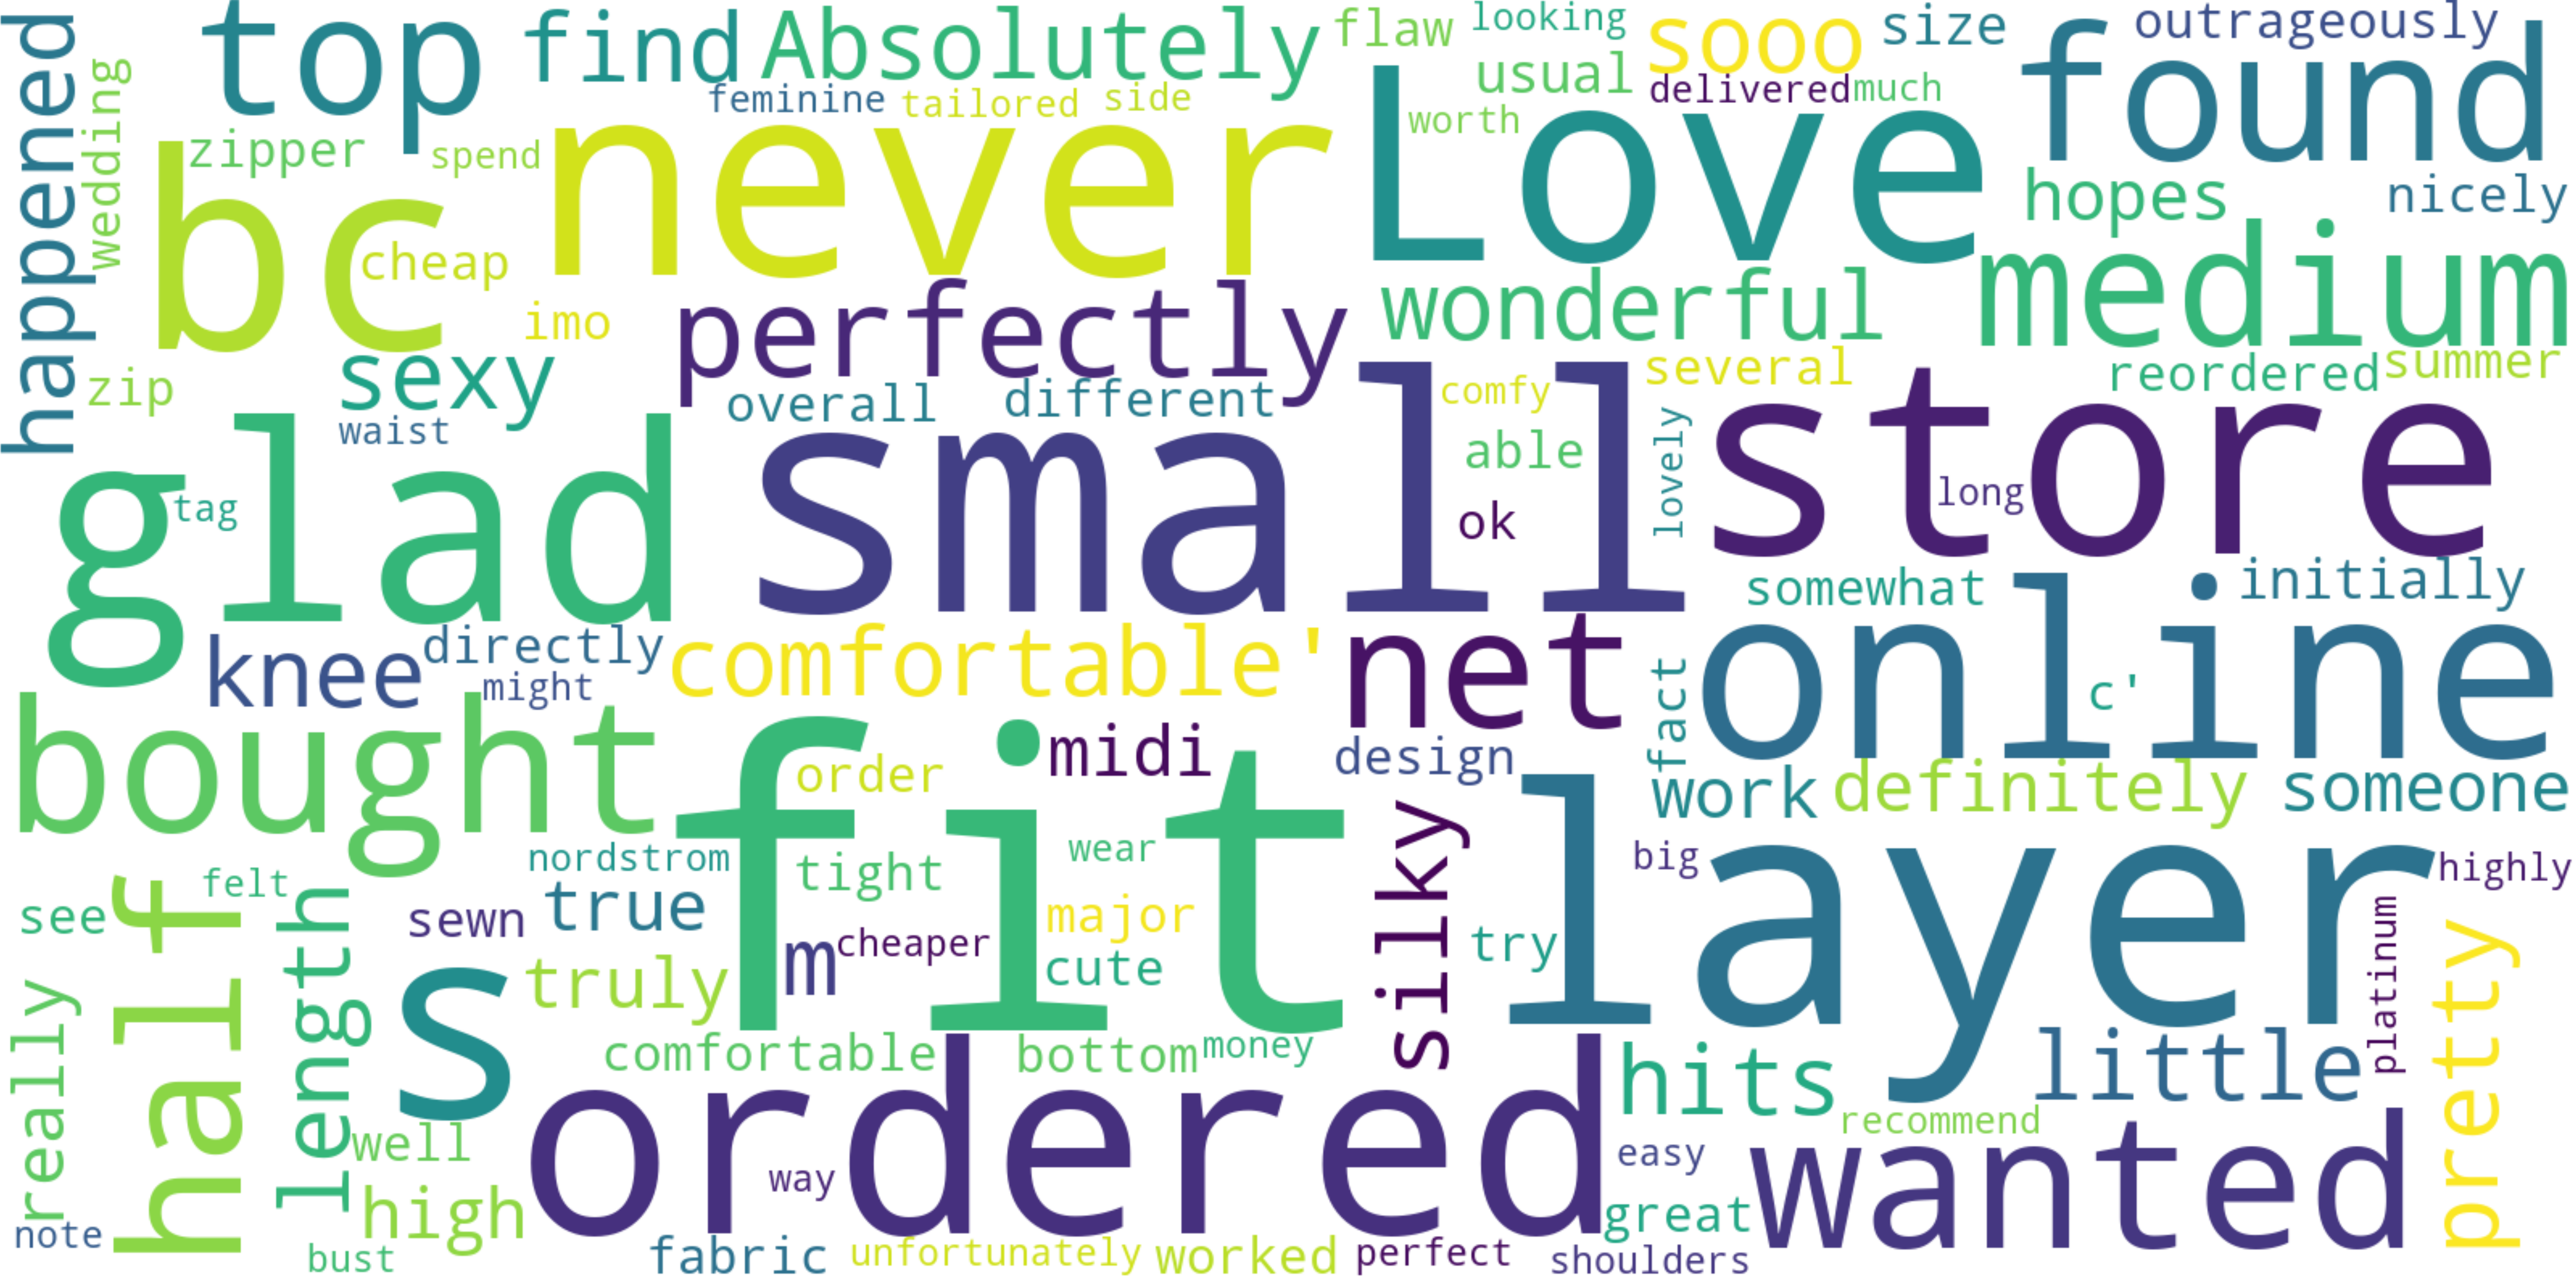
\includegraphics[width=0.7\linewidth]{cloud_ratehighly.png}
    \caption{高评分评论内容词云图}
    \label{cloud_ratehighly}
\end{figure}

​图~\ref{cloud_ratelow}描绘了低评价打分的Review Text-评论内容中出现频次多的词汇,出现了少量负面词汇,如narrowing、sadly、waiting等。

\begin{figure}[hbt!]
    \centering
    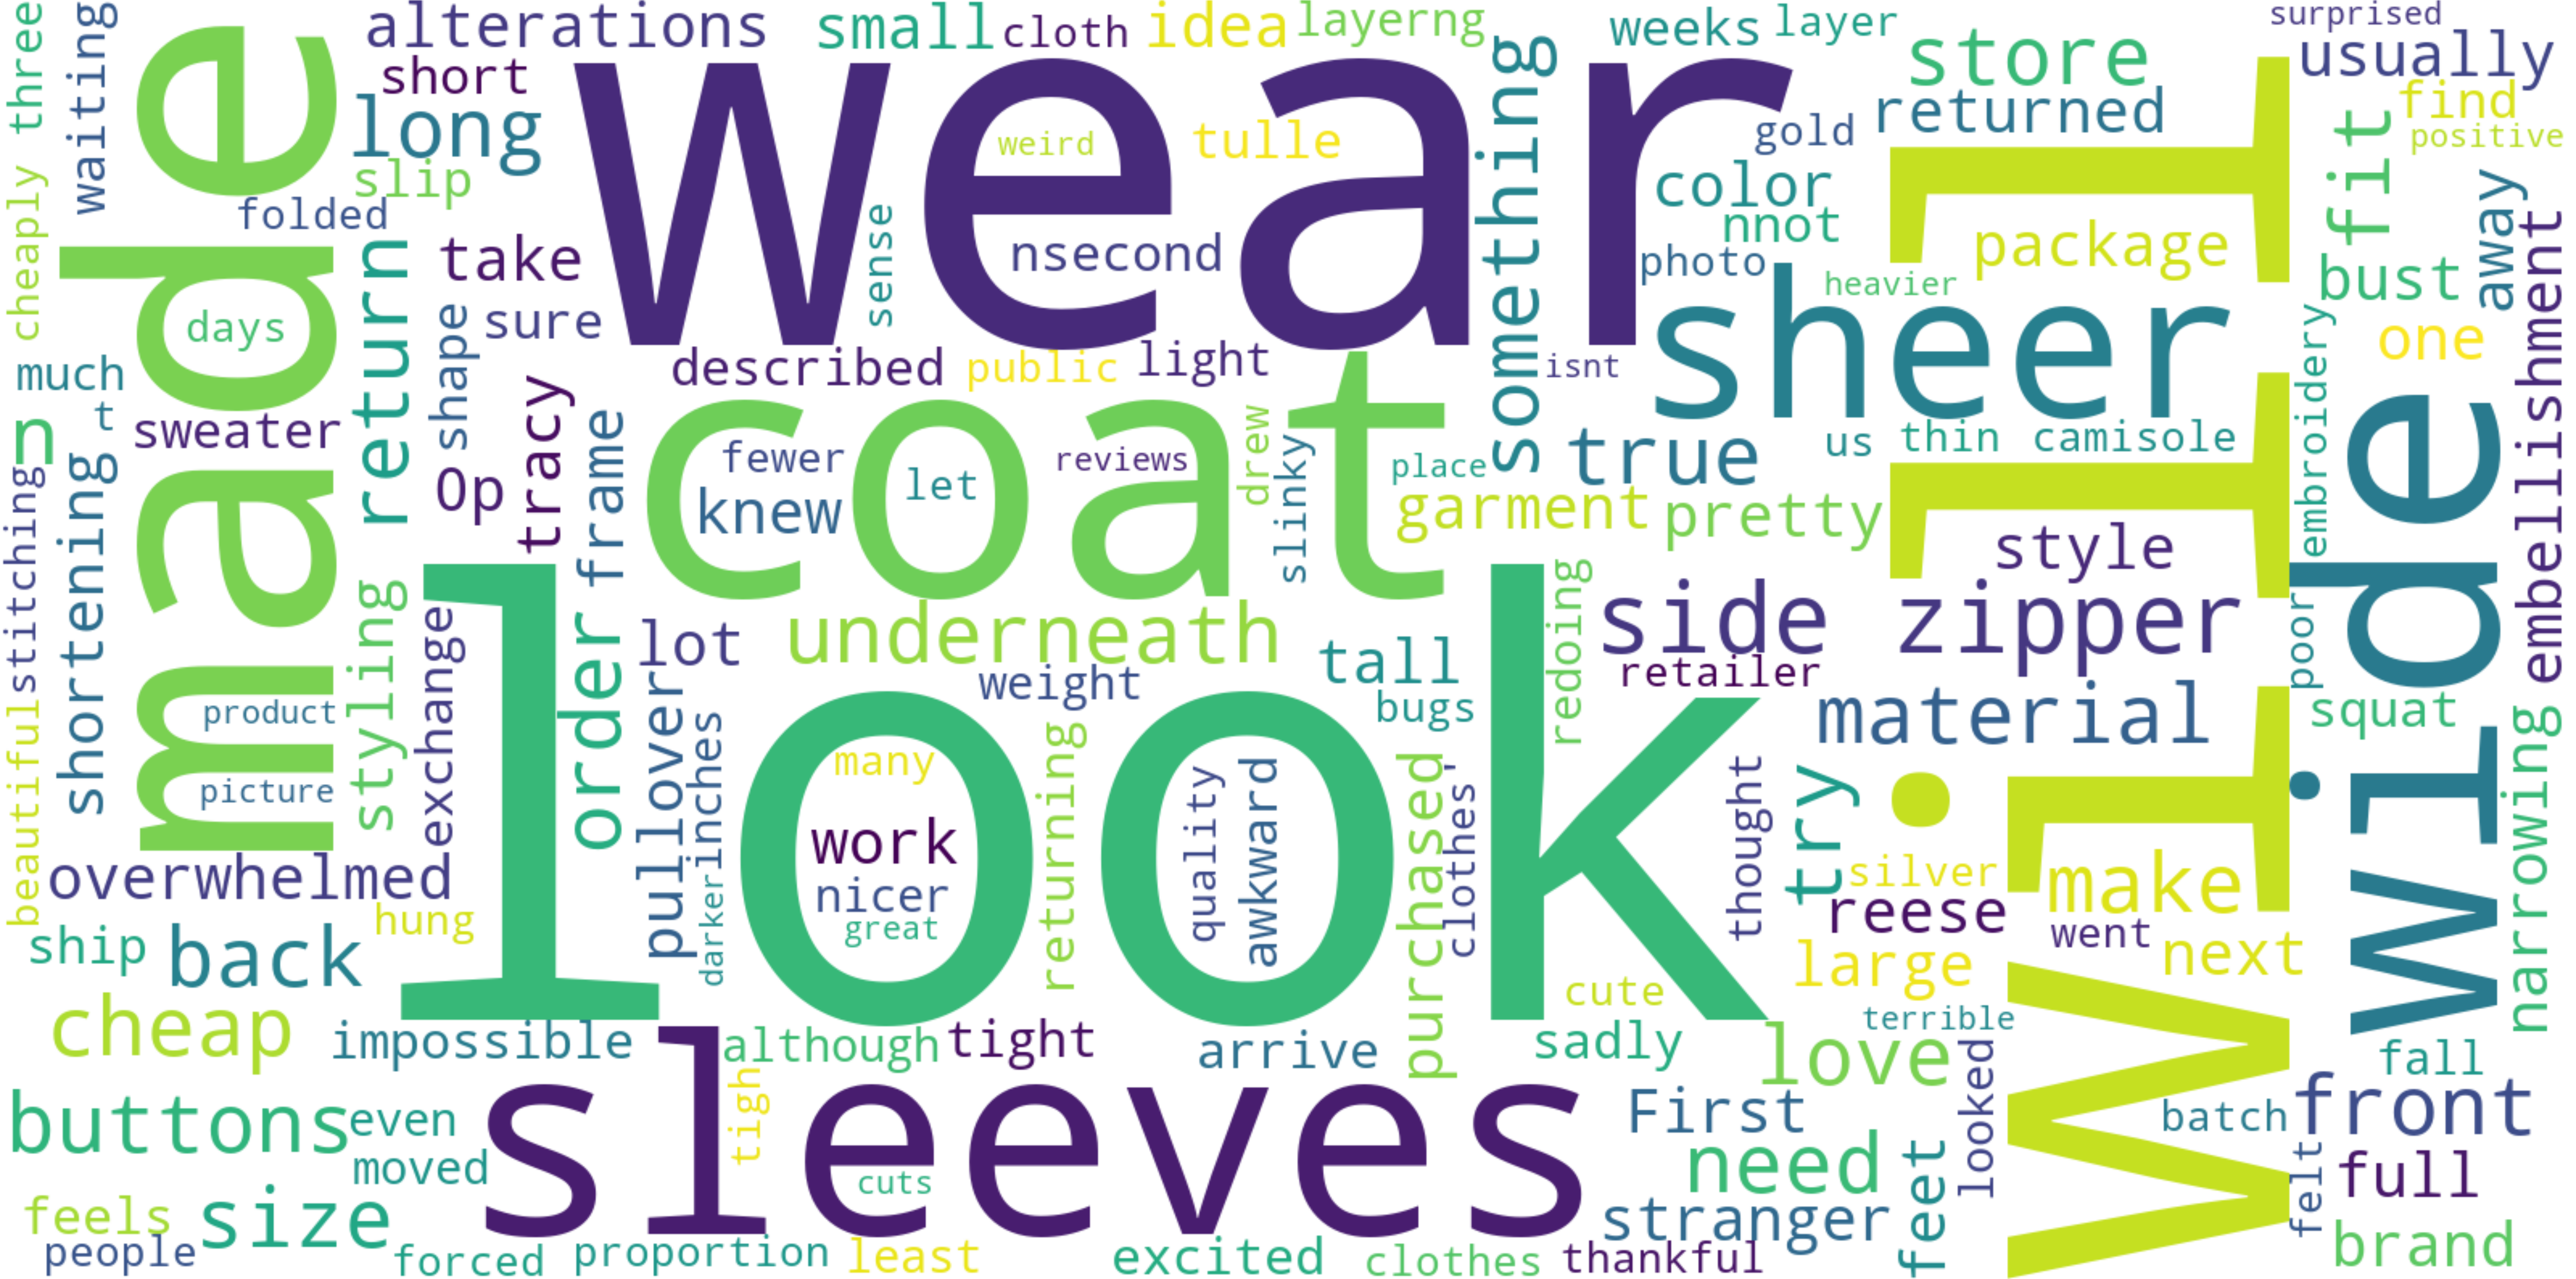
\includegraphics[width=0.7\linewidth]{cloud_ratelow.png}
    \caption{低评分评论内容词云图}
    \label{cloud_ratelow}
\end{figure}

\subsection{基于Losgistic算法的模型训练与评估}

\noindent$\bullet$\textbf{模型训练}

由于已经通过nltk自然语言处理工具包训练得到了评论内容的情感倾向,接下来我们想进一步探究评论内容与是否推荐之间的关系,即基于评论的内容训练出一个模型,推测出其是否有意愿将该产品推荐给好友,该模型将有助于我们判断在没有是否推荐属性时,人们的产品分享倾向,为之后的研究提供基础。

​对于评论文本,利用TF-IDF来提取文本特征,使用TfidfVectorizer 函数,将原始文本转换为tf-idf 特征矩阵,将 CountVectorizer 和TfidfTransformer的所有功能组合在一个模型中;之后利用sklearn库的traintestsplit函数划分训练集和验证集,最后利用Losgistic算法进行训练,由于losgistic算法中的参数对结果影响不大,在此使用默认参数训练。

\noindent$\bullet$\textbf{模型评估}

\noindent \textbf{准确度:}

Traindata Accuracy: 0.9128273118992376

Traindata ROC: 0.8887917239773266

Validationdata Accuracy: 0.8912947414935926

Validationdata ROC: 0.842036818826101

\noindent \textbf{分类评估报告:}

\begin{table}[hbt!]
    \begin{threeparttable}
    \caption{分类评估报告}
    \label{table_classification}
    \begin{tabular}{lllll}
    \toprule
    \headrow attribute & precision & recall & f1-score & support\\
    \midrule
    0(not Recommended) & 0.56 & 0.78 & 0.65 & 596 \\ 
    \midrule
    1(Recommended) & 0.96 & 0.91 & 0.94 & 3930 \\ 
    \midrule
    accuracy & & & 0.89  & 4526 \\ 
    \midrule
    macro avg & 0.76 & 0.84 & 0.79 & 4526 \\ 
    \midrule
    weighted avg & 0.91 & 0.89 & 0.90 & 4526\\ 
    \bottomrule 
    \end{tabular}
    \end{threeparttable}
\end{table}

\noindent \textbf{特征权重可视化:(基于eli5库)}

从图~\ref{feature_importance}我们可以发现,love为推荐标签最重要的特征向量,前三名特征向量都有积极的情感倾向;位于右列最底部的disappointed为影响不推荐标签权重最大的特征向量,但是仔细研究会发现,其中会有一些词汇如was、wanted等判断错误,说明模型还不是十分完备。

\begin{figure}[hbt!]
    \centering
    \includegraphics[width=0.5\linewidth]{feature_importance.png}
    \caption{特征重要性可视化}
    \label{feature_importance}
\end{figure}

\noindent \textbf{模型训练可视化分析}

\begin{figure}[hbt!]
    \centering
    \includegraphics[width=1.0\linewidth]{text.png}
    \caption{Losgistic算法下文本单词分析}
    \label{text}
\end{figure}

~\\
~\\
~\\

\subsection{基于lightgbm算法的模型训练与评估模型训练:}

\noindent$\bullet$\textbf{模型训练}

LightGBM是一款基于决策树算法的分布式梯度提升框架。为了满足工业界缩短模型计算时间的需求,LightGBM的设计思路主要是两点:(1)   减小数据对内存的使用,保证单个机器在不牺牲速度的情况下,尽可能地用上更多的数据;(2)   减小通信的代价,提升多机并行时的效率,实现在计算上的线性加速。由此可见,LightGBM的设计初衷就是提供一个快速高效、低内存占用、高准确度、支持并行和大规模数据处理的数据科学工具。

\noindent$\bullet$\textbf{模型评估}

train's auc: 1

valid's auc: 0.926843

F1 Score: 0.9365184109805992

\noindent \textbf{模型训练可视化分析}

\begin{figure}[hbt!]
    \centering
    \includegraphics[width=1\linewidth]{text2.png}
    \caption{lightgbm算法下文本单词分析1}
    \label{text2}
\end{figure}

\begin{figure}[t]
    \centering
    \includegraphics[width=1\linewidth]{text3.png}
    \caption{lightgbm算法下文本单词分析2}
    \label{text3}
\end{figure}

~\\
~\\
~\\
~\\
~\\
~\\
~\\

\section{结论与展望}

本文针对某女装电商平台的在线评论数据进行建模,对在线评论数据进行预处理工作,包括缺失值处理、特征生成与选择;通过单变量和多变量分布的探索,对数据有了进一步的了解,同时发掘了一些客户画像信息;通过VADER的情绪分析模型实现了对文本评论数据的倾向性判断以及关于主题的高频特征词提取,并且通过高频词的频率分析,进一步提炼客户情感,从而为商家今后发展策略和其他客户购买产品提供进一步的建议。最后,通过Logistic和Lightgbm算法,将评论文本向量化,预测其推荐产品的概率,为商家设计新的宣传营销策略提供了启示。

\section{参考文献}

[1]李杨,徐泽水,王新鑫.基于在线评论的情感分析方法及应用[J].控制与决策,2023,
38(02):304-317.DOI:10.13195/j.kzyjc.2022.1788.

[2]杨春晓,张鹤馨,黄家雯,等. 卷烟在线评论的文本情感分析[J]. 中国烟草学报,2020,26(2):92-100. 

[3]李宏媛,陶然. 服装电商评论情感分析研究[J]. 智能计算机与应用,2017,7(1):27-30,34. DOI:10.3969/j.issn.2095-2163.2017.01.007. 

[4]胡云凤. 基于主题模型的在线评论分析方法研究[D]. 陕西:西安电子科技大学,2017.
\end{document}